\label{sec:ipf}
This chapter describes how Individual Path Finding is formalized and how computation can be achieved using ASP and Clingo. 

\begin{figure}[H]
    \centering
    \caption{Overview of IPF}\label{fig:overview_ipf}
    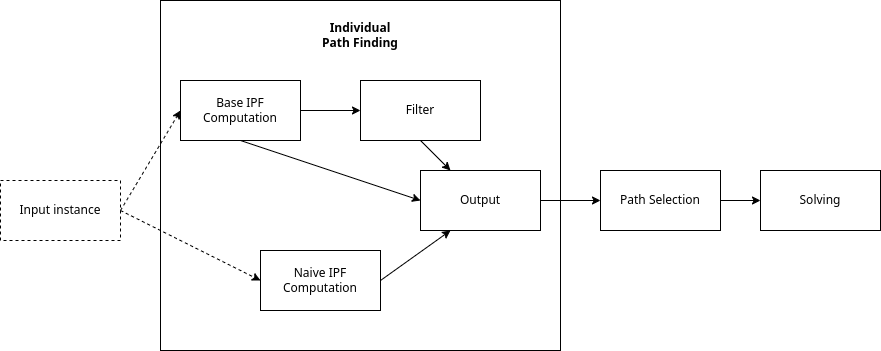
\includegraphics[width=\widthimg]{img/overview_ipf.drawio.png}
\end{figure}

\section{Formalization}

Individual Path Finding~\cite{luis2020plan,delling2009engineering} (IPF) represents the computation of multiple paths for each agent without considering collision in a given MAPF problem. The idea is then to use the paths for Plan Merging. We formalize IPF as a triple \((V,E,A)\) which is defined as in MAPF. The output is a non-empty set of set of paths \(\tau\). For each agent \(a \in A\), we have \(\tau[a]\) = \(\{\pi_0,\dots,\pi_n\}\). For lighter notation, we write \(\gamma_a = \tau[a]\), and also \(\gamma\) to refer to a set of path in general. Paths composing \(\gamma\) can be of different length. The following figure illustrate a \(\tau = \{\gamma_r, \gamma_b, \gamma_g\}\) where \(|\gamma_r|=3\), \(|\gamma_b|=1\) and  \(|\gamma_g|=1\). 

\begin{figure}[H]
    \centering
    \caption{Example of a \(\tau = \{\gamma_r, \gamma_b, \gamma_g\}\)}\label{fig:ipf_example}
    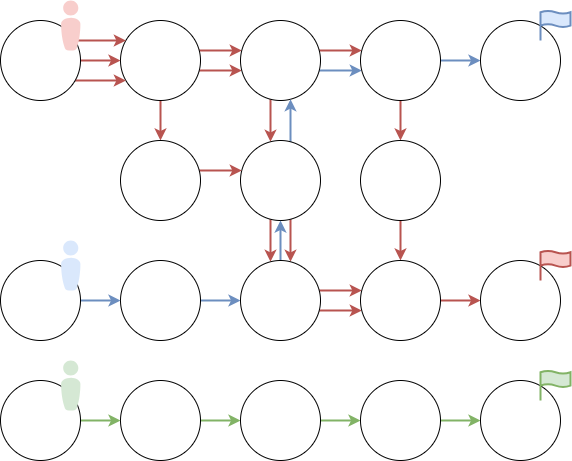
\includegraphics[width=\widthimg]{img/ipf_example.drawio.png}
\end{figure}


Paths can have different inner properties such as, length, number of bends, coverage of the graph or inter-connected properties such as number of plan conflict, diversity, distance and so on. The work achieved in the thesis has been made considering only length of paths, potential conflict, diversity and distance.

Path length is a very important property. We can splits paths into two length category; shortest paths, and non-shortest path.

\subsection{Diversity and Distance}

Diversity evaluates the variety of used vertices for a given set of paths of an agent. We introduce diversity as a sum of unique vertices visited at each time step. The function described in~\ref{math:diversity_formula} computes diversity for a given \(\gamma\).The formula is based on the Hamming distance~\cite{hanaka2022computing}. 

\begin{equ}[H]
    \begin{equation}\label{math:diversity_formula}
        distance(\gamma) = |\bigcup^{\pi \in \gamma}{(\cup^{v,t \in \pi}{(v,t)})}|
    \end{equation}
    \caption{Diversity function definition}
\end{equ}

Other diversity computation can be used, such as the Jaccard coefficient~\cite{habochal21a}. The difference between Jaccard coefficient and Hamming distance is that the first one focuses on the number of nodes that two paths have in common, while the second one focuses on the number of differences between the two paths. For our purpose, Hamming distance is more appropriate, however, it require that set are of the same length. Since paths in \(\gamma\) can be of different length, an adapted function was necessary. Note that the function~\ref{math:diversity_formula} do not gives an index that can be compared to other \(\gamma\)'s diversity. Furthermore, this equation is easy to implement with Clingo.

On the other hand, we can compute distance among paths in a \(\gamma\). Taken pair wisely, the distance between two paths is the sum of the distance between the vertices at each time step. Note that the distance between two vertices each be an arbitrary function such as euclidean distance or the shortest path length between these two vertices. We refer to this arbitrary function as \(dist(v,v')\). In our case, we consider \(dist(v,v')\) as the euclidean distance between \(v\) and \(v'\). The formalization of the distance for a given \(\gamma\) is defined in the following equation~\ref{math:distance_formula}. 

\begin{equ}[H]
    \begin{equation}\label{math:distance_formula}
        diversity(\gamma) = \mathlarger{\sum_{\pi,\pi' \in \gamma, \pi \neq \pi' }}{(\sum_{t=0}^{t \rightarrow min(|\pi|,|\pi'|)}{dist(\pi[t],\pi'[t])})}
    \end{equation}
    \caption{Diversity function definition}
\end{equ}


Figure~\ref{fig:diversity_vs_distance} shows two \(\gamma\) of size \(|\gamma|=2\). The first one shows an example of the most diverse \(\gamma\) possible for this problem (multiple solutions exist, and we consider paths in \(\gamma\) of same length). On the other side, we have an example of the most distant \(\gamma\) possible for this problem. Red squares illustrate the difference between diversity and distance.

\begin{figure}[H]
    \centering
    \caption{Diversity vs Distance}\label{fig:diversity_vs_distance}
    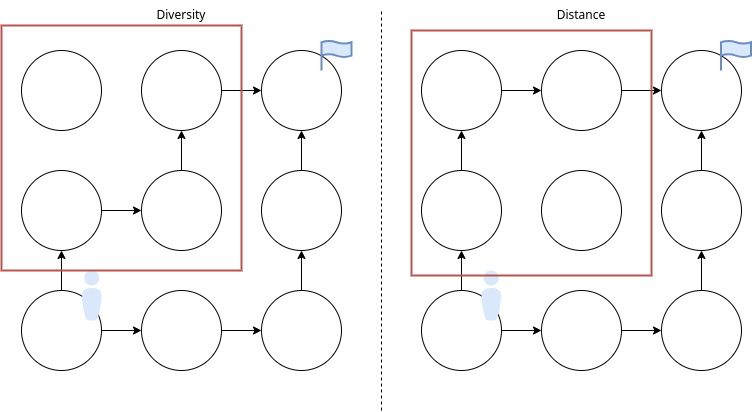
\includegraphics[width=\widthimg]{img/diversity_vs_distance.drawio.png}
\end{figure}



\section{Computation}


In this subsection, we present two different approaches for computing multiple paths. Even though IPF constitutes a side topic for this thesis, a concern was to be able to compute \(x\) paths for each agent within a reasonable time. We implemented the following computation approaches using Clingo (ASP). Computing paths with programming languages such as C, C++, Rust, and so on might offer better speed. We opted to stick with Clingo for its straightforwardness and technology consistency throughout this work. This section may serve as a starting point for future work on computing multiple paths using ASP and Clingo.

\subsection{Naive IPF Computation}\label{sec:naive_ipf_computation}

The first approach that we describe is a direct modification of the encoding presented in the section~\ref{sec:introduction}. The copy adds a new constant to the encoding called \textit{npaths} which denotes the number of paths to compute per agent. We modify \(at/3\) and \(move/4\) predicates, by adding a new argument being the identifier of the path. A unique path is now defined with an agent \(R\) and a path identifier \(I\). With these new directives, we obtain an encoding that we  call \textbf{Naive IPF}~\ref{lst:naive_ipf} which computes multiple paths for each agent in one call.

\begin{minipage}[H]{\linewidth}
\begin{lstlisting}[style=mystyle, caption={Naive IPF computation}, label={lst:naive_ipf}, numbers=left, ,escapechar=|]
    agent(R,1..npaths) :- agent(R). |\label{line:agent_id_and_path_id}|
    
    at(R,I,P,0) :- start(R,P), agent(R,I).

    time(1..horizon).
    {move(R,I,U,V,T) : edge(U,V)} 1 :- agent(R,I), time(T). |\label{line:move4_to_move5}|

    at(R,I,V,T) :- move(R,I,_,V,T). |\label{line:at3_to_at4}|
    :- move(R,I,U,_,T), not at(R,I,U,T-1).

    at(R,I,V,T) :- 
        at(R,I,V,T-1), 
        not move(R,I,V,_,T),
        time(T).

    :- { at(R,I,V,T) }!=1 , agent(R,I), time(T). 

    :- goal(R,V), not at(R,I,V,horizon).
\end{lstlisting}
\end{minipage}

The encoding in Listing~\ref{lst:naive_ipf} has the exact same principles as the base MAPF encoding (see Listing~\ref{lst:base_mapf_encoding}). Line~\ref{line:agent_id_and_path_id} introduces id \(I\) for paths. Note that in this case, all agents would have the same number of paths. We could use other predicates to describe how many paths are required for each agent of an instance. Lines~\ref{line:move4_to_move5} and~\ref{line:at3_to_at4} shows predicates \textit{move/4} and \textit{at/3} getting changed to predicates \textit{move/5} and \textit{at/4} now including the ID of paths.


The main flaw that comes with the encoding described is slowness. Requesting multiple paths per agent raises the search-space considerably. Even if we remove conflict consideration in the encoding,  the grounder needs to ground the rules containing predicate \(move/5\) at most \(|A| * npaths\) time. In addition, more variables induce a slower solving. 
However, this encoding gives us the opportunity to add properties to paths. For example, to implement diversity\ref{math:diversity_formula}, we can use an optimization statement:

\begin{minipage}[H]{\linewidth}
\begin{lstlisting}[style=mystyle]
    #maximize{1,R,V,T : at(R,I,V,T)}.
\end{lstlisting}
\end{minipage}

More definitive additions such as constraining specific paths of specific agents to have a defined length, a defined number of bends and so on, could be used.
Another flaw that comes with this encoding is that there is no guarantee that all paths for the same agent are different. However our \textbf{Naive IPF} encoding would still compute the requested number of paths for this agent \(a\) even though paths are the same. This can be fixed using collision for individual agents; the risk could be to revert to classical MAPF solving.

\subsection{Base IPF computation}\label{sec:base_ipf_computation}

By using multi-shot solving and assumptions~\cite{karoscwa21a}, it is  possible to ground both predicates \(at\) and \(move\) once for all agents. To do so, we tweak the naive IPF encoding described in section~\ref{sec:naive_ipf_computation} and obtain the encoding in Listing~\ref{lst:base_ipf}. This encoding can be interpreted as simple pathfinding that will be executed one agent at a time. Furthermore, \(start/2\) and \(goal/2\) predicates are not necessary; these are handled by assumptions.


\begin{minipage}[H]{\linewidth}
\begin{lstlisting}[style=mystyle, caption={Base IPF computation}, label={lst:base_ipf}]
    time(1..horizon).

    {at(V,0) : vertex(V)} = 1.

    { move(U,V,T) : edge(U,V)} 1 :- time(T).

    at(V,T) :- move(_,V,T).
    :- move(U,_,T), not at(U,T-1).

    :- { at(V,T) } != 1, time(T).

    at(V,T) :- at(V,T-1), not move(V,_,T), time(T).

    current_agent(R) :- at(V,0), start(R,V). |\label{line:identify_current_agent}|
    at(GV,T) :- at(GV,T-1), time(T), goal(R,GV), |\label{line:stay_after_goal_reached}| 
             current_agent(R). 
\end{lstlisting}
\end{minipage}

Line~\ref{line:identify_current_agent} aims to identify the current agent the solver is generating paths for. Through the assumption of the predicate \(at/2\) at time step 0, we can retrieve the current agent using the corresponding \(start/2\) predicate. Line~\ref{line:stay_after_goal_reached} is then designed to guarantee that once the path of an agent reaches its goal, the agent remains at its goal location.


The flowchart described in figure~\ref{fig:flowchart_ipf_computation} illustrates the process of base IPF computation. It first ground the instance with the encoding, then solve with the start and goal positions of an agent as assumptions. Finally, it extends \textit{at/2} with agent ID and model number. We use the model number to identify different paths of the same agent; the model enumeration represents different possible assignations for the problem. Requesting \(n\) models means requesting \(n\) paths for an agent.

\begin{figure}[H]
    \centering
    \caption{Flowchart of IPF computation using multi-shot solving and assumption}\label{fig:flowchart_ipf_computation}
    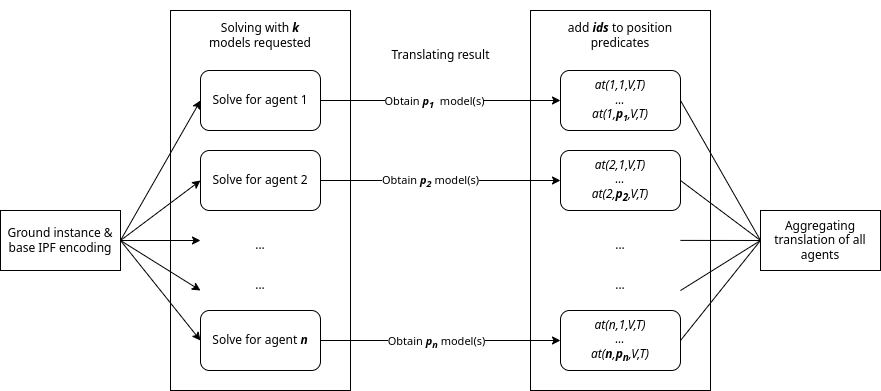
\includegraphics[width=\widthimg]{img/flowchart_ipf_computation.drawio.png}
\end{figure}


We define \(1 \leq p \leq k\), if solving an instance with \(k\) requested models, the number of possible models \(p\) can be lower. 
We use a Python wrapping to control and manage assumptions. A pseudocode of the wrapper is denoted in Listing~\ref{lst:pseudo_code_ipf_wrapper}

\begin{minipage}[H]{\linewidth}
\begin{lstlisting}[style=mystyle, caption={Pseudo code of base IPF encoding wrapper}, label={lst:pseudo_code_ipf_wrapper}, numbers=left, ,escapechar=|]
    result |\(\leftarrow\)| list()
    ground(instance + base IPF encoding)

    for each agent in instance |\{|
        assume(initial and goal position)
        solve()

        for each model |\{|
            translate `at/2'|\(\rightarrow\)|`at/4'
            add translation to result
        |\}|
    |\}|  
\end{lstlisting}
\end{minipage}

A nice property that comes with this approach is that since we use model enumeration to create different paths, if Clingo enumerates fewer models than requested, we can assume that there are no other paths possible of this length.

Base IPF computing reduces computation time significantly; given the way Clingo works, decomposing the problem into one agent at a time and reusing grounding works is faster than trying to solve multiple problems at once. It does, however, compute random paths. In order to compute the shortest paths, we can use the optional predicates described in list~\ref{list:instance_format_explanation_part2}. Assumptions allow us to force \(goal/2\) predicate to be reached a specific time step,  We can then change the goal position assumption and force it to be reached at a certain time step instead of at the horizon. We can use the same principle to compute paths of different lengths for one agent; this requires an additional solving and translation step.

Furthermore, in this process, we can compute additional paths with a modified time step associated with the goal. This addition enables agents to reach their destination xx time steps later than the originally defined duration. This strategy proves valuable when a limited number of paths are computed, as it provides the IPF solver with extra possibilities to generate additional paths.

Given the way base IPF computation works, it seems difficult to assign different properties to the paths that depends on other paths. Properties, such as, length, number of bends can easily be achieve. On the other hand, diversity and distance seems difficult. To achieve a similar result, we can request a large number of paths and create a subset out of them that satisfy chosen properties. 






\subsection{Filters}

Compared to naive IPF computation, properties depending on other paths seem difficult to compute. We can however create subset of previously computed \(\gamma\) by filtering paths given some criteria. A filter \(f\) is defined as such; \( f(\gamma) \subseteq \gamma \). We introduce two criteria functions. The first being a function selecting \(k\) most diverse paths following~\ref{math:diversity_formula} and the second one a function selecting \(k\) most distant paths following~\ref{math:distance_formula}.

\begin{minipage}[H]{\linewidth}
\begin{lstlisting}[style=mystyle, caption={Encoding of diverse filter}, label={lst:diversity_filter}, numbers=left, ,escapechar=|]
    #const npath = 5.

    {dpath(R,I): at(R,I,_,_)} npath :-  agent(R). |\label{line:div_select_path_p1}|
    #maximize {1@2,R,I : dpath(R,I)}. |\label{line:div_select_path_p2}|
    
    dpath(R,I,V,T) :- dpath(R,I), at(R,I,V,T). |\label{line:div_retrieving_pos}|
        
    #maximize {1@1R,V,T : dpath(_,_,V,T)}. |\label{line:maximizing_diversity}|
\end{lstlisting}
\end{minipage}

The diversity encoding in Listing~\ref{lst:diversity_filter} starts by picking, for each agent, at most \textit{npath} paths among all path available denoted in line~\ref{line:div_select_path_p1}. Line~\ref{line:div_select_path_p2} maximize the amount of chosen paths. Using this optimization statement, we avoid unsat results when not enough paths exist for an agent. Line~\ref{line:div_retrieving_pos} retrieves positions and time steps of selected paths. From these selected path, we can count the tuple \((V,T)\) and maximize them with the optimization statement in line~\ref{line:maximizing_diversity}.

\begin{minipage}[H]{\linewidth}
\begin{lstlisting}[style=mystyle, caption={Encoding of distance filter}, label={lst:distance_filter}, numbers=left, ,escapechar=|]
    #const npath = 5.

    {dpath(R,I): at(R,I,_,_)} npath :-  agent(R). |\label{line:dist_select_path_p1}|
    #maximize {1@1,R,I : dpath(R,I)}. |\label{line:dist_select_path_p2}|
    
    dpath(R,I,V,T) :- dpath(R,I), at(R,I,V,T).|\label{line:dist_retrieving_pos}|
         
    dist(R,I1,I2,T, (X1-X2)*(X1-X2) + (Y1-Y2)*(Y1-Y2)) :- |\label{line:dist_computing_distance}|
        dpath(R,I1,(X1,Y1),T),  
        dpath(R,I2,(X2,Y2),T), I1!=I2. 

    dsum(R,DS) :- |\label{line:dist_intermediate}|
        DS=#sum{D:dist(R,I1,I2,_,D), dpath(R,I1), dpath(R,I2)}, 
        agent(R).

    #maximize {1@2,D : dsum(R,D)}.|\label{line:maximize_distance}|
\end{lstlisting}

\end{minipage}


The distance encoding Listing~\ref{lst:distance_filter} starts by picking for each agent, at most \textit{npath} paths among all path available, maximizing the number of selected path and then retrieving their position and time step (from line~\ref{line:dist_select_path_p1} to~\ref{line:dist_retrieving_pos}). Line~\ref{line:dist_computing_distance} introduces a new predicate \(dist/4\) which denotes  euclidean distance of two different paths of the same agent. We then have an intermediate rule line \ref{line:dist_intermediate} which sums the distance of paths for each agents. It is then used in the optimization statement in line~\ref{line:maximize_distance} to maximize the distance issued by \(D\).